


% See "book", "report", "letter" for other types of document.

\documentclass[12pt,a4paper,headsepline,bibliography=totoc,listof=totoc,headinclude=false,footinclude=false,BCOR5mm]{scrreprt} % use larger type; default would be 10pt

\usepackage[latin1]{inputenc} % set input encoding (not needed with XeLaTeX)
 \usepackage{hyperref}
\usepackage{url}


%%% PAGE DIMENSIONS

 

 
%%% PACKAGES
\usepackage{a4,german,booktabs}
\usepackage[lmargin=3cm, rmargin=3cm]{geometry}
\usepackage{amsmath,amssymb}
%\usepackage{fancyhdr}




 
\usepackage{array} % for better arrays (eg matrices) in maths
\usepackage{paralist} % very flexible & customisable lists (eg. enumerate/itemize, etc.)
\usepackage{verbatim} % adds environment for commenting out blocks of text & for better verbatim
\usepackage{subfig} % make it possible to include more than one captioned figure/table in a single float
\usepackage{graphicx}
 \usepackage[tc]{titlepic}


% These packages are all incorporated in the memoir class to one degree or another...

%%% HEADERS & FOOTERS
\usepackage{fancyhdr} % This should be set AFTER setting up the page geometry
\pagestyle{plain} % options: empty , plain , fancy
%\renewcommand{\headrulewidth}{0pt} % customise the layout...



%%% SECTION TITLE APPEARANCE
\usepackage{sectsty}
\allsectionsfont{\sffamily\mdseries\upshape} % (See the fntguide.pdf for font help)
% (This matches ConTeXt defaults)

%%% ToC (table of contents) APPEARANCE
%\usepackage[nottoc,notlof,notlot]{tocbibind} % Put the bibliography in the ToC
\usepackage[titles,subfigure]{tocloft} % Alter the style of the Table of Contents
\renewcommand{\cftsecfont}{\rmfamily\mdseries\upshape}
\renewcommand{\cftsecpagefont}{\rmfamily\mdseries\upshape} % No bold!

%%% END Article customizations

%%% The "real" document content comes below...







\begin{document}
\begin{titlepage}
\thispagestyle{empty}
 \begin{center}
 \begin{figure}[htbp]
    \centering
    \subfloat{
\includegraphics[width=0.4\textwidth]{feulogo}}\hspace{7.5em}
     \subfloat{
\includegraphics[width=0.375\textwidth]{wiwilogo}}\\
 \centering
  \vspace*{1.0cm}
    \subfloat{
\includegraphics[width=0.75\textwidth]{rechtsfoto}}
\end{figure}

   


  %\vspace*{1.5cm}

  \vspace*{2.5cm}
 {\bf \Large Bewertung von Optionen und zustandsbedingten Anspr{\"u}chen (contingent claims) mit der Feynman-Kac-Formel}
 \vspace*{3.5cm} \\
 {\Large Seminararbeit\\von\\}
 \vspace{0.5cm}
 {\large \bfseries Corvin Idler\\}
c/o European Commission, Delegation Australia, Diplomatic Pouch, \\1049 Brussels, BELGIUM\\
 +61 2 6271 2777, idler@uni-koblenz.de
 \vfill



\begin{table}[h]
	\centering
	\begin{tabular}{|l| l|}\hline
		Studiengang & Bachelor Wirtschaftswissenschaften\\ \hline
		Betreuer & Prof. Dr. Hermann Singer\\ \hline
		Matrikelnummer & 7529953\\ \hline
		Arbeit vorgelegt am: & 22.10.2010\\ \hline
	\end{tabular}
\end{table}

 \end{center}
\end{titlepage}
\tableofcontents


 
\chapter{Einleitung}
Die vorliegende Arbeit besch\"aftigt sich mit der Bewertung von zustandsbedingten Anspr\"uchen (auch als  zufallsbehaftete Finanzpositionen, Eventualforderungen oder contingent claims bezeichnet) unter Anwendung der sogenannten Feynman-Kac Formel. Dabei wird \"uberwiegend Bezug auf die Bewertung von Aktienoptionen als Anwendungsfall genommen, was darauf zur\"uckzuf\"uhren ist, dass diese Kategorie von Eventualforderungen ausgiebigst in der wissenschaftlichen Literatur beschrieben ist. Es soll jedoch der Eindruck vermieden werden, dass die besprochenen Formalismen und Modelle ausschlie{\ss}lich f\"ur diesen Anwendungsfall Relevanz besitzen. Vielmehr sind sie die Grundlage f\"ur die Bewertung einer Vielfalt von zufallsbehafteten Finanzpositionen. Beispielsweise werden in \cite{Zaglauer2006} Ans\"atze f\"ur die Bewertung gemischter Kapitallebensversicherungen mit einem \"ahnlichen mathematischen und modelltechnischen Instrumentarium, wie dem hier vorgestellten, aufgezeigt. Nach einer allgemeinen Beschreibung des finanzmathematischen Modells in Kapitel \ref{fmm}, werden in Kapitel  \ref{FK} L\"osungsm\"oglichkeiten des Bewertungsproblemes mittels der Feynman-Kac Formel aufgezeigt, sowie die Grenzen der Anwendbarkeit des vorgestellten Formalismus besprochen.

\chapter{Finanzmathematisches Modell}\label{fmm}
\section{Preisprozesse f\"ur Basiswert und Bond}\label{preisp}
F\"ur die L\"osung des Bewertungsproblems von zustandsbedingten Anspr\"uchen ist die Modellierung des (Preis)Prozesses des zugrunde liegenden Basiswertes (underlying) eine Grundvoraussetzung.
Die folgenden Ausf\"uhrungen seien beschr\"ankt auf eine in der Finanzmathematik (speziell im Kontext der Aktienoptionsbewertung) weit verbreitete Modellklasse, bei der die Kursentwicklung des Basiswertes durch folgende stochastische Differentialgleichungen beschrieben werden \cite[S. 141]{Lin2006}:
 \begin{equation} \label{generalunderlying}
X(t) = \overbrace{X(0) + \underbrace{\int_0^t \! \alpha(s,X(s)) \, ds}_{\text{Riemann-Integral}} + \underbrace{\int_0^t \! \sigma(s,X(s)) \, dW(s)}_{\text{Ito-Integral}}}^{\text{Ito-Prozess}}, 0 \leq t \leq T \end{equation}
  \begin{equation} \label{diffgeneralunderlying}
dX(t)=  \alpha(t,X(t)) \, dt +  \sigma(t,X(t)) \, dW(t) \end{equation}
Dabei symbolisiert $W(t)$ eine Brownsche Bewegung und die beiden Funktionen $\alpha(t,X(t))$ und $\sigma(t,X(t))$ stehen f\"ur die Drift, respektive die Volatilit\"at des stochastischen Prozesses $X(t)$. Die M\"oglichkeit von Dividendenzahlungen wird im Kontext dieser Arbeit aus \"Ubersichtlichkeitsgr\"unden ausgeschlossen, eine Modellierung ist jedoch prinzipiell ohne weiteres m\"oglich. Wie in Abschnitt \ref{arb} ersichtlich wird, ist f\"ur das Bewertungsproblem noch die Modellierung des Preisprozesses einer risikofreien Anlage (Bond) $B(t)$ in Abh\"angigkeit des Zinssatzes $r(t,X(t))$ erforderlich, welche in ihrer allgemeinsten Form wie folgt lautet: 
  \begin{equation} \label{bond}
dB(t) = B(t)r(t,X(t))dt; B(0)=1 \end{equation}

Eine spezifische Auspr\"agung des mit Gleichung (\ref{generalunderlying}) bis (\ref{bond}) beschriebenen Modells ist z.B. das von Black-Scholes \cite{Black73} in welchem die Wertentwicklung $X(t)$ eines Basiswertes mittels {\bf geometrischer} Brownscher Bewegung mit {\bf konstanter Volatilit\"at} \begin{math}\sigma(t,X(t))=\sigma\end{math},  {\bf konstanter Drift} \begin{math}\alpha(t,X(t))=\alpha\end{math} und {\bf konstantem risikolosem Zinssatz} \begin{math}r(t,X(t))=r\end{math} modelliert wird:
\newpage

  \begin{equation} \label{underlying}
dX(t) =  \alpha X(t) \, dt +  \sigma X(t) \, dW(t) \end{equation}

  \begin{equation} \label{underlying1}
W(t+\tau) - W(t) \sim N(0, \sqrt{\tau}) \end{equation}
  \begin{equation} \label{bond1}
dB(t) = B(t)r dt; B(0)=1 \end{equation}
Mittels Ito-Integral \"uber die Brownsche Bewegung ergibt sich folgender Zusammenhang \cite[S.146]{Lin2006}

  \begin{equation} \label{underlying2}
ln X(t) = ln X(0) + (\alpha - \frac{\sigma^{2}}{2})t + \sigma W(t) \end{equation}
bzw.
  \begin{equation} \label{underlying3}
X(t) =  X(0) e^{(\alpha - \frac{\sigma^{2}}{2})t + \sigma W(t)} \end{equation}

Die gemachten Annahmen implizieren u.a. dass sich der Basiswertkurs im Zeitverlauf kontinuierlich entwickelt (keine Kursspr\"unge), die Kursver\"anderungen im Zeitablauf unkorreliert sind und die logarithmierten Inkremente normalverteilt sind\footnote{letzteres ergibt sich aus der {\bf geometrischen} Brownschen Bewegung} \cite[S.4]{Zimmermann2000}\cite{Osborne59}. 

Neben dem Black-Scholes Model, dessen Annahme einer konstanten Volatilit\"at in der Realit\"at selten zutrifft,  sind noch eine Vielfalt von weitaus weniger restriktiven Modellauspr\"agungen in der Literatur beschrieben. Diese Ans\"atze sehen zeitliche Schwankungen der Volatilit\"at vor und modellieren sie als einen eigenst\"andigen (oft von einer Brownschen Bewegung getriebenen) stochastischen Prozess.
Eine tabellarische Aufstellung verschiedener Volatilit\"atsprozesse findet sich in \cite[S. 212]{Singer1999}.  Verbreitet sind vor allem Modelle welche sich Ornstein-Uhlenbeck-Prozessen in vielf\"altiger Form bedienen \cite{Javaheri2002}. Fuer die Zwecke dieser Arbeit sei exemplarisch der Ansatz von \cite{Nelson1992} herausgegriffen, welcher sich von dem GARCH\footnote{generalized autoregressive conditional heteroskedasticity}-Formalismus aus dem Bereich der Zeitreihenanalyse ableitet. Die Stochastizit\"at der Volatilit\"at wird dabei \"uber folgenden Prozess hergestellt:
 \begin{equation} \label{vola}
d \ \text{log} \ \sigma(t)^2 =\lambda \ ( \text{log} \ \sigma(t)^2 - \text{log} \ \bar{\sigma})dt + \gamma dV(t)
\end{equation}
Der Parameter $\gamma$ symbolisiert dabei die Volatilit\"at der Volatilit\"at, $\lambda$ wird oft als Steifigkeit\footnote{speed of mean reversion} und $ \bar{\sigma}$ als Gleichgewichtsniveau\footnote{mean reversion level} bezeichnet. Getrieben wird der Prozess von der Brownschen Bewegung $dV(t)$ welche mit der Brownschen Bewegung des Basiswertes korreliert sein kann ($Var(dW, dV) = \rho dt$).
\section{Bewertung durch Duplikationsportfolios}\label{arb}
Das Preismodell f\"ur die Bewertung von zustandsbedingten Anspr\"uchen welches innerhalb dieser Arbeit verwendet wird, basiere auf der Annahme eines perfekten Finanzmarktes  \cite[Kap. 4.1]{Franke2004} :
  \begin{itemize}
\item Abwesenheit von Arbitragem\"oglichkeiten
\item keine Transaktionskosten
\item keine Steuern 
\item short-selling uneingeschr\"ankt  m\"oglich
\item Soll- und Habenzinsen identisch
\item Wertpapiere beliebig teilbar
  \end{itemize}

Obige Modellannahmen sind von zentraler Bedeutung in Bezug auf die Bewertung von Optionen und anderen zustandsabh\"angigen Anspr\"uchen durch sogenannte Duplikationsportfolios. Dabei synthetisiert man den zu bewertenden Finanztitel $C(X,t)$ (mit noch unbekanntem Wert) - durch Kauf und Verkauf anderer am Markt umlaufender Titel - mit einem Portfolio $V(X,t)$ (mit bekanntem Wert/Preis) in einer Art und Weise, dass beide Portfolios zu einem bestimmten Zeitpunkt $T$ wertgleich sind ($C(X,T) = V(X,T)$). Durch kontinuierliche Umschichtungen innerhalb des Duplikationsportfolios werden in diesem Modell Wertver\"anderungen w\"ahrend der Laufzeit des zu bewertenden Finanztitels gleichwertig nachgebildet ($dC(X,t) = dV(X,t)$), sodass beide Portfolios auch zu jedem davor liegenden Zeitpunkt $t\le T$ wertgleich sind ($C(X,t) = V(X,t)$). Diese Umschichtungen werden ohne positiven oder negativen externen Cash Flow vorgenommen, was man als Selbstfinanzierungsbedingung  bezeichnet \cite[S.7]{Zimmermann2000}. Durch diese dynamische Hedging-Strategie ergibt sich der Wert des Finanzderivats zu jedem Zeitpunkt $t$ anhand des Wertes des Duplikationsportfolios. Das Duplikationsportfolio $V(X,t)$ z.B. f\"ur eine Aktienoption $C(X,t)$ besteht gew\"ohnlich aus $\Delta(X,t)$ Aktien und einem Festgeld bzw. risikolosen Zerobond $B(X,t)$) mit dem Zinsatz $r$ \cite[S.5]{Zimmermann2000}:

\begin{equation} \label{repli}
C(X,t) = V(X,t)=\Delta(X,t)X+B(X,t)\end{equation}

Innerhalb dieses mathematischen Formalismus dr\"ucken sich die kontinuierlichen Umschichtungsoperationen im Duplikationsportefolio zum Zwecke der Wertanpassung durch folgende Wahl  aus: $\Delta(X,t) = \frac{\partial C(X,t)}{  \partial X}$ (perfekte Replikation ohne Residualrisiko).

\section{Fundamentale partielle Differentialgleichung (FPD)}\label{FPD}
Alle oben genannten Modellannahmen f\"uhren kombiniert letztlich zu der {\bf fundamentalen partiellen Differenzialgleichung der Optionspreisbildung}, welche auch als verallgemeinerte Black-Scholes-Differentialgleichung\cite[S. 222 ff]{Singer1999} oder dynamische Hedginggleichung \cite{Zimmermann2000} bezeichnet wird. Sie lautet in ihrer allgemeinen Form:
 \begin{equation} \label{fpdefk}
\begin{split}
\frac{\partial C(X,t)}{\partial t} + \frac{\partial C(X,t)r(X,t)}{\partial X}+
\frac{\partial^{2} C(X,t) \sigma^{2}(X,t)}{2\partial^{2} X}  - r(X,t)C(X,t) = 0;  \\ C(X,T) = G(X_{T}), 0 \leq t \leq T\end {split}\end{equation}

Eine genaue Herleitung von Gleichung (\ref{fpdefk}) findet sich in \cite[S. 222 ff]{Singer1999} \cite{Zimmermann2000} \cite{Franke2004}. Eine bedeutende Eigenschaft sei hervorgehoben: die obige Gleichung ist vollkommen unabh\"angig von der Drift $\alpha (X,t)$ des Basiswertprozesses aus Gleichung (\ref{generalunderlying})! Dies ist darauf zur\"uckzuf\"uhren, dass die perfekte dynamische Hedgingstrategie aus Abschnitt \ref{arb} eine Beziehung zwischen Optionspreis und Basiskurs herstellt, welche v\"ollig frei von jeglichen Risikopr\"aferenzen ist \cite{Cox1975} und somit den risikolosen Zinssatz $r$ als Bezugsrendite inne hat. Dieses Ph\"anomen l\"asst sich in letzter Instanz (mittelbar \"uber unterstellte Linearit\"at der Nutzenfunktionen der Marktteilnehmer) auf die Annahme der Arbitragefreiheit zur\"uckf\"uhren \cite[S. 336]{Merton2003}\cite[S. 153]{Cox1976}\cite{Harrison1981} und ist auch als Fundamentaltheorem der Verm\"ogensbewertung\footnote{Fundamental Theorem of Asset Pricing} und Bewertungsregelrepr\"asentationstheorem\footnote{Pricing Rule Representation Theorem} bekannt \cite[S.9]{Philip2003} \cite{Schachermayer2008}.

Gleichung (\ref{fpdefk}) gilt f\"ur sich genommen f\"ur beliebige zustandsbedingte Anspr\"uche, deren Wert nur von $X$ und $t$ abh\"angen. Die {\bf spezifische Auszahlungsstruktur} $G(X_{T})$ der Finanzderivate zum F\"alligkeitszeitpunkt fliesst nicht in die Gleichung selbst mit ein, sondern wird in Form von Randbedinguneng formuliert und zur L\"osung der Gleichung herangezogen. Beispielsweise gelten f\"ur eine europ\"aische Long-Call Option\footnote{Kauf einer Kaufoption}  die folgenden Randbedingungen: 
\begin{equation}\label{longcall}
C(X,T) = G(X_{T}) = \max[0,X_{T}-K]
\end{equation}
und 
\begin{equation} 
C(X,t) \geq  0
\end{equation}
wobei $K$ den Aus\"ubungspreis der Option symbolisiere.
In der Regel l\"asst sich Gleichung (\ref{fpdefk}) nur f\"ur bestimmte Spezialf\"alle analytisch l\"osen. Eine Vielzahl von eleganten L\"osungsm\"oglichkeiten er\"offnen sich durch Anwendung der Feynman-Kac Formel, welche im Folgenden Kapitel besprochen wird.

\chapter{Feynman-Kac Formel}\label{FK}
\section{Feynman-Kac L\"osungsansatz der FPD}
In ihrer allgemeinsten Form bezieht sich die Feynman-Kac Gleichung \cite{Feynman1948,Kac1949} auf die L\"osung der Schr\"odinger-Gleichung in der Quantenphysik. Eine Spezialisierung dieser Gleichung ergibt sich, wenn man sie auf (\ref{diffgeneralunderlying}) und (\ref{fpdefk}) anwendet. Die vorliegende Problemstellung (das Finden einer L\"osung f\"ur die FPD) wird mit Hilfe der Feynman-Kac Gleichung  wie folgt angegangen:
\begin{equation} \label{feynman}
C(X,t) = E \left [e^{- \int_{t}^{T}  r(X(s),s)ds} G(X(T)) \mid X(t) = X \right ] 
\end{equation}  In diesem Formalismus ist der Wert einer Option also der zum Zeitpunkt $t$ abdiskontierte Erwartungswert (bzgl. eines bestimmten Wahrscheinlichkeitsma{\ss}es\footnote{risikoneutrales Bewertungsma{\ss}}) der Auszahlung eines zustandsbedingten Anspruches in Abh\"angigkeit von dem Preis $X$ des underlying zum Zeitpunkt $t$ \cite{Brandimarte2006}. 
Innerhalb obiger Modellierung ist es von zentraler Bedeutung, welche Pfade in dem vorliegenden dynamischen stochastischen System m\"oglich sind. Man definiert ein Ma{\ss} \"uber der Menge aller m\"oglichen Pfade vom Anfangszustand $X(t)=X$ zum Endzustand $X(T)$. Dies erm\"oglicht mittels Pfad\-integral \"uber alle m\"oglichen Pfade von $X(t)=X$ nach $X(T)$ die Berechnung von Erwartungswerten von pfadabh\"angigen Funktionalen, wie z.B. der Auszahlungsstruktur $G(X_{T})$ einer Option. Pfadintegrale nennt man auch sum-over-histories (Pfade) oder  funktionale Integrale \cite[S. 129ff.]{Linetsky1998}. Offensichtlich ist die bedingte Dichte $p(X_T\mid X)$  von fundamentalem Interesse f\"ur diesen Formalismus, wie im folgenden Abschnitt deutlich wird. 

\section{Berechnungsbeispiele} 
\subsection{Anwendungsf\"alle mit analytischer L\"osung} \label{anwendung}
Ein klassisches Rechenbeispiel f\"ur die Feynman-Kac Gleichung, bei welcher diese  eine analytische L\"osung besitzt, ist eine europ\"aische Long-Call Option in einer Black-Scholes-Welt (d.h. mit unterstellter geometrischer Brownscher Bewegung f\"ur den Preisprozess des Basiswertes, sowie einem konstantem Zinssatz).
Wie in Gleichung (\ref{longcall}) bereits beschrieben, gilt f\"ur die Auszahlungsstruktur dieser Option $G(X_{T}) = \max[0,X_{T}-K]$. Die Feynman-Kac-Formel erh\"alt in diesem Szenario folgende Gestalt:
\begin{equation} \label{feynmanbs}\begin{split}
C(X,t) &=e^{-r(T-t)}  E \left [\max[X_{T}-K,0] \mid X(t) = X \right ]  \\ &= e^{-r(T-t)}  \int_{K}^{\infty} (X_{T}-K) p(X_{T}\mid X)dX_{T} \\ &= e^{-r(T-t)} \left[ \int_{K}^{\infty} X_{T} p(X_{T}\mid X)dX_{T} -K\int_{K}^{\infty} p(X_{T}\mid X)dX_{T} \right]
\end{split}
\end{equation}
Den Modellannahmen entsprechend (vgl. insbesondere Gleichung (\ref{underlying3})) ist $X_{T}/X=e^x$ mit folgender Verteilung \cite[S. 240]{Singer1999}:
\begin{equation}\label{vert}  x \sim N(\nu, \gamma^2) ; \upsilon = (r - \frac{\sigma^2}{2})(T-t), \gamma^2 = \sigma^2(T-t)
\end{equation}
In Analogie zu Abschnitt \ref{FPD} wird auch hier  $\alpha = r$ gesetzt. Durch den Zusammenhang aus Gleichung (\ref{vert}) kann die bedingte Dichte $p(X_T\mid X)$ \"uber die Normalverteilungsdichtefunktion $\phi()$ wie folgt bestimmt werden: 
\begin{equation}\label{beddicht} \frac{1}{\sqrt{2 \pi \gamma^2}} \exp  \frac{(x-\nu)^2}{-2\gamma^2}  =\phi(x; \nu,\gamma^2)dx = p(X_T\mid X)dX_T
\end{equation} Eine genaue Herleitung findet sich in \cite[S. 134 ff]{Linetsky1998}.
Dies erm\"oglicht Gleichung (\ref{feynmanbs}) wie folgt umzuformen:
\begin{equation} \label{feynmanbsII}\begin{split}
C(X,t) &= e^{-r(T-t)} \left[ \int_{K}^{\infty} X_{T} p(X_{T}\mid X)dX_{T} - K \int_{K}^{\infty} p(X_{T}\mid X)dX_{T} \right] \\
&=e^{-r(T-t)} \left[ \underbrace{\int_{\log(K/X)}^{\infty} Xe^{x} \phi(x; \nu,\gamma^2)dx}_{I_1} - K \underbrace{\int_{\log(K/X)}^{\infty} \phi(x; \nu,\gamma^2)dx}_{I_2} \right]
\end{split}\end{equation}
Die Integrale $I_1$ und $I_2$ in dieser Gleichung k\"onnen unter unter Zuhilfenahme der Verteilungsfunktion der Normalverteilung $\Phi()$ folgenderma{\ss}en aufgel\"ost werden {\cite[S. 203ff]{Hausmann2002}:}
\newpage

\begin{equation} \label{feynmanbsIII}\begin{split}
&C(X,t)\\ &=e^{-r(T-t)} \left[ \int_{\log(K/X)}^{\infty} Xe^{x} \phi(x; \nu,\gamma^2)dx - K \int_{\log(K/X)}^{\infty} \phi(x; \nu,\gamma^2)dx \right] \\
&=e^{-r(T-t)} \left[ \int_{\log(K/X)}^{\infty} X\exp(x) \frac{1}{\sqrt{2 \pi \gamma^2}} \exp \left ( \frac{(x-\nu)^2}{-2 \gamma^2} \right )dx - K I_2 \right]\\
&=e^{-r(T-t)} \left[X \int_{\log(K/X)}^{\infty}  \frac{1}{\sqrt{2 \pi \gamma^2}} \exp \left ( \frac{(x-\nu)^2}{-2\gamma^2} + x\right ) dx - K I_2 \right] \\
&=e^{-r(T-t)} \left[X \int_{\log(\frac{K}{X})}^{\infty}  \frac{1}{\sqrt{2 \pi \gamma^2}} \exp \left ( \frac{(x-\nu)^2}{-2\gamma^2} + x - (\nu + \frac{\gamma^2}{2})+ (\nu + \frac{\gamma^2}{2})\right ) dx- K I_2 \right]\\
&=e^{-r(T-t)} \left[X \int_{\log(\frac{K}{X})}^{\infty}  \frac{1}{\sqrt{2 \pi \gamma^2}} \exp \left ( \frac{(x-\nu)^2 -2\gamma^2x +2\gamma^2(\nu + \frac{\gamma^2}{2})}{-2\gamma^2} + (\nu + \frac{\gamma^2}{2})\right ) dx- K  I_2 \right] \\
&=e^{-r(T-t)} \left[X \int_{\log(\frac{K}{X})}^{\infty} e^{\nu + \gamma^{2}/2} \frac{1}{\sqrt{2 \pi \gamma^2}} \exp \left ( \frac{(x-\nu)^2 -2\gamma^2x +2\gamma^2\nu + \gamma^4)}{-2\gamma^2} \right ) dx- K I_2 \right]  \\
&=e^{-r(T-t)} \left[Xe^{\nu + \gamma^{2}/2}  \int_{\log(K/X)}^{\infty} \frac{1}{\sqrt{2 \pi \gamma^2}} \exp \left ( \frac{(x-(\nu+\gamma^2))^2}{-2\gamma^2} \right ) dx- K I_2 \right] \\
&=e^{-r(T-t)} \left[Xe^{\nu + \gamma^{2}/2} \int_{\log(K/X)}^{\infty}  \phi(x; \nu+\gamma^2,\gamma^2)dx - K  I_2 \right]  \\
&=e^{-r(T-t)} \left[Xe^{\nu + \gamma^{2}/2} \int_{\log(K/X)}^{\infty}  \phi(x; \nu+\gamma^2,\gamma^2)dx - K \int_{\log(K/X)}^{\infty} \phi(x; \nu,\gamma^2)dx \right] \\
&= e^{-r(T-t)} \left[Xe^{\nu + \gamma^{2}/2}  \left (1- \Phi(\log(K/X); \nu+\gamma^2,\gamma^2) \right ) - K (1-\Phi(\log(K/X); \nu,\gamma^2))\right] \\
&= e^{-r(T-t)} \left[Xe^{\nu + \gamma^{2}/2}  \Phi(\underbrace{\frac{\log(X/K) + \nu+\gamma^2}{ \gamma}}_{d_1 = d_2 + \gamma}) - K \Phi(\underbrace{\frac{\log(X/K) + \nu}{ \gamma}}_{d_2})\right] 
\end{split}\end{equation}
 Durch eine  h\"aufig vorgenommene und in Gleichung (\ref{feynmanbsIII}) angedeutete Substituierung der beiden Verteilungsfunktionsausdr\"ucke, wird weiter vereinfacht zu:
\begin{equation} \label{feynmanbseinf}\begin{split}
C(X,t) =e^{-r(T-t)} \left[ Xe^{\nu + \gamma^{2}/2}  \Phi(d_1) - K \Phi(d_2) \right] \\
\end{split}\end{equation}
Eine Resubstituierung von $\nu$ und $\gamma$ f\"uhrt letztlich zu der Black-Scholes Formel:
\begin{equation} \label{BS}\begin{split}
C(X,t) =X\Phi(d_1) - e^{-r(T-t)} K \Phi(d_2)  \\
\end{split}\end{equation}
Wie man sehen kann, sind f\"ur die Berechnung einer einfachen europ\"aischen (plain vanilla) Long-Call-Option folgende Parameter von N\"oten:

  \begin{itemize}
\item der Aus\"ubungspreis $K$ der Option
\item der Kurs bzw. Preis $X(t)$ des Basiswertes zum Bewertungszeitpunkt $t$
\item der Zinssatz $r$ 
\item die (Rest)Laufzeit (T-t) der Option
\item die (angenommene) Volatilit\"at des Basiswertes bezogen auf den Bewertungszeitraum (Laufzeit)
  \end{itemize}
Bis auf die Volatilit\"at d\"urfte zwischen zwei Marktteilnehmern Einvernehmen \"uber die oben aufgelisteten Parameter bestehen, da sie exogen vorgegeben sind. In diesem Sinne reduziert sich die Preisfindung in diesem Kontext auf die H\"ohe der Volatilit\"at des Basiswertes welche man f\"ur den Betrachtungszeitraum zugrunde legt.
Will man die in Abschnitt \ref{fmm} schon angesprochene M\"oglichkeit stochastischer Volatilit\"aten in den Feynman-Kac Formalismus miteinbeziehen, so sind die Parameter $\nu$, $\gamma$ und somit auch $d_1$ und $d_2$ entsprechend anzupassen. Geht man beispielsweise von einem Preisprozess f\"ur den Basiswert mit stochastischer Volatilit\"at aus, welcher den folgenden Gesetzm\"a{\ss}igkeiten folgt,

 \begin{equation} \label{stochvola}dX(t)=  rX(t) \, dt +  \sigma(t)X(t) \, \left [ \sqrt{1-\rho^2}dW(t)  + \rho dV(t)\right ]
\end{equation}

\begin{equation} \label{stochvola2}d\sigma(t)=  a(t,\sigma(t)) \, dt +  b(t,\sigma(t)) \, dV(t) 
\end{equation}
dann ergeben sich laut \cite[S. 242]{Singer1999} die Variablen $\nu$ und $\gamma$ wie folgt:
  \begin{equation} \label{nu}
\nu = r(T-t) - \frac{1}{2} \int_t^T \sigma^2 ds + \rho \int_t^T \sigma dV
\end{equation}
  \begin{equation} \label{gamma}
\gamma^2 = (1-\rho^2) \int_t^T \sigma^2 ds 
\end{equation}
Dementsprechend sind die die Terme $d_1$ und $d_2$ f\"ur diesen Fall wie folgt definiert:
  \begin{equation} \label{d2}
d_2 =\frac{ \log(X/K)+ r(T-t) - \frac{1}{2} \int_t^T \sigma^2 ds + \rho \int_t^T \sigma dV}{\sqrt{(1-\rho^2) \int_t^T \sigma^2 ds}}
\end{equation}

  \begin{equation} \label{d1}
d_1 =\frac{ \log(X/K)+ r(T-t)+ (\frac{1}{2}-\rho^2) \int_t^T \sigma^2 ds + \rho \int_t^T \sigma dV}{\sqrt{(1-\rho^2) \int_t^T \sigma^2 ds}}
\end{equation}
Die resultierende Preisformel f\"ur eine Long-Call-Option ist jetzt nicht mehr nur auf den Kurs des Basiswertes zum Bewertungszeitpunkt bedingt, sondern auch auf den Wert der Volatili\"at des Basiswertes zum Bewertungszeitpunkt. Formal dr\"uckt sich das wie folgt aus:

 \begin{equation} \label{fkstoch}\begin{split}
C(X,\sigma,t) =X E\left[ e^{\rho \int_{t}^{T} \sigma dV -\frac{1}{2} \rho^2\int_{t}^{T}\sigma^2(s)ds} \Phi(d_1) \mid X(t) = X, \sigma(t) = \sigma \right] - \\ 
e^{-r(T-t)}K E\left[\Phi(d_2) \mid X(t) = X, \sigma(t) = \sigma \right] 
\end{split}
\end{equation}


\subsection{Verfahren f\"ur Anwendungsf\"alle ohne analytische L\"osung} 
Szenarien ohne analytische L\"osung m\"ussen mittels numerischer Methoden approximiert werden. Aus der Vielzahl der m\"oglichen Verfahren \cite{Singer1999}\cite{Fries2007} seien in dieser Arbeit Monte Carlo Simulationen als Verfahren zur numerischen Integration exemplarisch herausgegriffen. Bei diesen Verfahren werden in der Regel als erster Schritt eine gro{\ss}e Zahl von Pfaden des Basiswertes zufallsgeneriert. Dies ist insbesondere f\"ur die Bewertung von pfadabh\"angigen Optionen eine Grundvoraussetzung, da deren Auszahlungsfunktion per definitionem nicht ausschlie{\ss}lich (wenn \"uberhaupt) vom Preis des Basiswertes zum F\"alligkeitszeitpunkt abh\"angt, sondern vielmehr von einem, mehreren oder allen $X(t)$ w\"ahrend der Laufzeit der Option.  Es ist unumg\"anglich, dass bei der Anwendung von Monte Carlo Methoden ein \"Ubergang von der stetigen Modellierung zu einer diskreten Berechnung mit diskreten Zeitschritten $\delta t$ stattfindet, wie im Folgenden in Anlehnung an \cite{Brandimarte2006, Fries2007} am Beispiel von Gleichung (\ref{generalunderlying}) verdeutlicht:
  \begin{equation} \label{generalmonte}
X(t_{i+1}) =  X(t_i) +  \alpha(t_i,X(t_i))  \delta t_i  +  \sigma(t_i,X(t_i)) \delta dW(t_i) \end{equation}
Die Zufallsvariablen $dW(t_i)$ der einzelnen Zeitschritte $t_i$ sind dabei definitionsgem\"a{\ss} voneinander unabh\"angig. Solche Simulationen sind heutzutage selbst mit Standard-Tabellen\-kalkulationssoftware problemlos m\"oglich %\footnote{vgl. \url{http://www.bionicturtle.com/dloads/LO\%2014.x\%20Monte\%20CarloDemo.xls}}
\cite{Chance2004} \cite{Harper2008}. Neben der Restlaufzeit $(T-t)$ und den Funktionalen f\"ur Volatilit\"at $\sigma(t,X(t))$ und Drift $\alpha(t,X(t))$, sind die Monte Carlo Simulationen \"uber die Schrittweite(n) $\delta t_i$ bzw. die Anzahl $n$ der diskreten Zeitschritte, sowie die Anzahl $N$der simulierten Pfade parametrisiert, welche beide die Genauigkeit der Simulationsergebnisse steuern. Eine Simulation l\"a{\ss}t sich formal wie folgt beschreiben \cite[S.187]{Fries2007}:
  \begin{equation} \label{generalmontepfad}
X(t_{i+1},\omega_j) =  X(t_i,\omega_j) +  \alpha(t_i,X(t_i,\omega_j))  \delta t_i  +  \sigma(t_i,X(t_i,\omega_j)) \delta dW(t_i,\omega_j) \end{equation}
wobei $\omega_j$ den j-ten Pfad kennzeichnet. Somit ist die Gesamtsimulation des stochastischen Prozesses X gegeben durch die Menge
  \begin{equation} \label{menge}
\left \{ X(t_{i},\omega_j) \mid i=0,1, ...,n; j=1,...,N \right \} 
\end{equation}
F\"ur die Praxis ist bei der Parametrisierung darauf zu achten, auf welche Zeiteinheit sich Drift und Volatilit\"at beziehen, sofern sie denn konstant sind. Offensichtlich ist es h\"ochst bedeutsam, ob man zum Beispiel von einer j\"ahrlichen oder einer t\"aglichen Rendite von 10\% spricht. Sofern es sich bei Drift und Volatilit"at um Jahreswerte handelt, m\"ussen die Zeitschritte $\delta t_i$ in Jahresbruchteilen ausgedr\"uckt sein, um sicherzustellen dass die Simulation ein einheitliches zeitliches Bezugssystem hat.
F\"ur  Umrechnungen zwischen Jahres- und Tageswerten werden in der Regel nur die Anzahl der Handelstage ($\sim$252) ber\"ucksichtigt. In Abbildung \ref{pic1} und \ref{pic2} sind zwei Simulationsergebnisse mit $N=25$ f\"ur 10 Tage  geometrischer Brownscher Bewegungen graphisch dargestellt. Bei den angegebenen Werten f\"ur Volatilit\"at und Drift handelt es sich um Jahreswerte.
\begin{figure}[h!]
    \centering
    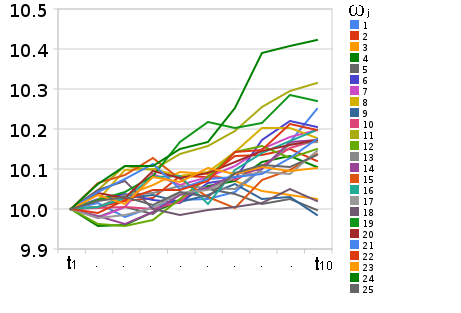
\includegraphics[width=0.90\textwidth]{1}
\caption{Simulierte Pfade diskretisierter Brownscher Bewegungen mit \\ $X_{t_1}=10, \alpha=55\%, \sigma=5\%, n=10$}\label{pic1}
\end{figure}
\begin{figure}[h!]
    \centering
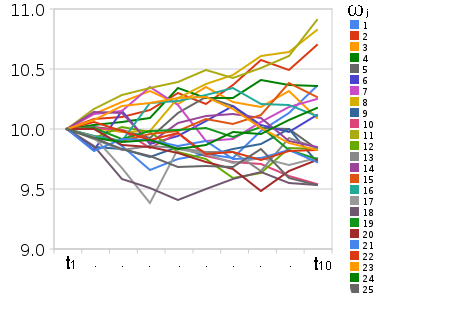
\includegraphics[width=0.90\textwidth]{2}\caption{Simulierte Pfade diskretisierter Brownscher Bewegungen mit \\ $X_{t_1}=10, \alpha=12\%, \sigma=20\%, n=10$}\label{pic2}
\end{figure}

Die M\"achtigkeit richtig angewendeter Monte Carlo Simulationen besteht darin, dass der Erwartungswert von nahezu beliebigen Funktionalen $f$ bez\"uglich potentiell aller Werte einer Trajektorie $X(s), t \leq s \leq T$ zum Beispiel durch:
   \begin{equation} \label{ewert}
E(f(X(t_{0}) ... X(t_{n})) =  \frac{1}{N} \sum_{j=1}^{N} f(X(t_0,\omega_j) ... X(t_n,\omega_j)) \end{equation}
approximiert werden kann. Beispielsweise f\"uhrt diese Methode bezogen auf das Szenario aus Kapitel \ref{anwendung}  zu folgendem L\"osungsansatz:
   \begin{equation} \label{bsp}
E(f(X(t_{0}) ... X(t_{n})) = E\left [\max[X_{T}-K,0] \mid X(t) = X \right ] =  \frac{1}{N} \sum_{j=1}^{N} X(t_n,\omega_j) - K) \end{equation}
 Auch eine Kombination von analytischen und Monte Carlo Methoden ist denkbar und verbreitet. So kann zum Beispiel bei der Kategorie der schwach pfadabh\"angigen knock-in Optionen das Erreichen des Schwellkurses $X_S$ Monte-Carlo-simuliert und anschlie{\ss}end der Preis (der durch Erreichen der Kursschwelle aktivierten Option) analytisch mittels der Black-Scholes Formel \cite[S. 447]{Brandimarte2006} \cite{Broadie97} berechnet werden. Daf\"ur wird in der Regel eine Indikatorfunktion $I(X)$ wie folgt definiert:
\begin{equation} \label{indi}
I(X)=\begin{cases} 1 & \text{falls  $\exists$ i \text{mit} $X(t_i) > X_S$} \\ 0 & \text{sonst}\end{cases} 
\end{equation}
Im Falle einer knock-in Calloption ergibt sich f\"ur den Preis somit folgender Zusammenhang
\begin{equation} \label{indi}
C(X,t) =e^{-rt*}  E \left [I(X)\max[X_{T}-K,0] \mid  X(t*) \right ]  
\end{equation}
Dabei symbolisiert $X(t*)$ den Kurs nach Detektion der Schwellkurs\"uberschreitung\footnote{bei kontinuierlicher Detektion gilt $X(t*)$ = $X_S$} und $t*$ den Detektionszeitpunkt. Man berechnet also den Wert der Option ab dem Zeitpunkt der Schwell\"uberschreitung mittels der klassischen Black-Scholes Formel und zinst diesen Betrag danach noch zum Bewertungszeitpunkt ab. Diesen Vorgang f\"uhrt man zum Zwecke der Erwartungswertbildung vielfach durch, wobei das \"Uberschreiten des Schwellkurses $I(X)$ und somit auch der \"Uberschreitungszeitpunkt $t*$ jeweils Monte Carlo simuliert wird.

\section{Grenzen der Feynman-Kac Formel} 
Die Grenzen des in dieser Arbeit besprochenen Formalismus werden \"uberwiegend durch die vorgenommen Modellannahmen aufgezeigt. Dies betrifft zum Beispiel die in Kapital \ref{arb} gemachten Annahmen bez\"uglich des perfekten Finanzmarktes, insbesondere die der Arbitragefreiheit. Es ist offensichtlich, dass der Bewertungsmechanismus in sich zusammen f\"allt, wenn die wesentlichen Annahmen bez\"uglich des Marktes nicht erf\"ullt sind. Am problematischsten erscheint in diesem Zusammenhang die Annahme von identischen Soll- und Habenzinsen.
Beschr\"ankend wirkt vor allem auch die Form der in Kapitel \ref{preisp} beschriebenen stochastischen Prozesse aus, die insbesondere keine Kursspr\"unge zulassen. Um der Realit\"at in diesem Zusammenhang etwas n\"aher zu kommen, m\"ussen Modelierungsans\"atze mit Sprungprozessen herangezogen werden. Auch die Annahme der Normalverteilung der Aktienkursrenditen ist \"au{\ss}erst problematisch, da empirische Untersuchungen darauf hinweisen, dass Verteilungsfunktionen f\"ur Ertr\"age von Finanzanlagen oft eine, im Vergleich zur Normalverteilung, hohe Kurtosis aufweisen \cite{Erben2006}. Ausserhalb des Bereiches reiner Aktienoptionen ist noch eine viel gr\"ossere Abweichung von der Normalverteilung, in Form h\"oherer oder niedrigerer Kurtosis oder auch negativer Schiefe, zu beobachten \cite[S. 377ff]{Busak2006}.
Dadurch f\"ande in der Praxis eine Unter- bzw. \"Ubersch\"atzung bzw. -bewertung des sogenannten Fat-Tail-Risikos (bzw. Chance) statt.
Erstaunlich ist in diesem Zusammenhang, dass in der Praxis gelegentlich die Annahme der log-Normalverteilung sowohl im Zusammenhang mit Aktienoptionen als auch mit Index-Optionen auf Aktienindizes angewandt wird. Dass dabei eine gewichtete Summe (Index) von log-normalverteilten Zufallsgr\"o{\ss}en ebenfalls einer log-Normalverteilung folgen soll, ist mathematisch schwer einzusehen.  
Letztlich muss es f\"ur die Anwendbarkeit des Feynman-Kac Formel m\"oglich sein, die in Kapitel \ref{FK} besprochenen \"Ubergangswahrscheinlichkeiten anzugeben oder zu simulieren. Je komplexer das zu bewertende Finanzprodukt oder Portfolio ist, desto schwieriger kann das sein. Diese Problematik wird schon bei der relativ geringf\"ugigen Modell\"anderung in Form stochastischer Volatilit\"aten deutlich, wie in Kapitel \ref{anwendung} beschrieben. Ein Beispiel f\"ur die Schwierigkeit selbst relativ intuitive Finanzprodukte zu bewerten, sind die massiven Probleme vor denen Versicherungsgesellschaften bei der Bewertung gemischter Kapitallebensversicherungen stehen \cite{Zaglauer2006}. Aber auch die Bewertung von komplexen Vertr\"agen im Rahmen von Mitarbeiteroptionsprogrammen ist alles andere als trivial, da juristische Details mathematisch abgebildet werden m\"ussen. Diese und \"ahnliche Problemstellungen sind Gegenstand aktueller Forschungen in der Finanz- und Aktuarwissenschaft. Ebenfalls nicht unkompliziert ist die Bewertung von contingent claims auf einen Basiswert (underlying), welcher selber nicht handelbar ist und es somit nicht zul\"asst die Eventualforderung \"uber ein Replikationsportfolio nachzubilden. Beispiele hierf\"ur sind Wetterderivate oder Volatilit\"ats-Swaps.


\interlinepenalty10000
\bibliographystyle{alphaurl}
\bibliography{biblio}

\end{document}
